\chapter{A highland maize chromosomal inversion decreases flowering time in a phosphorus-independent manner and leads to minor perturbations of the leaf phosphorus starvation response transcriptome.}
\label{chap-four}
\newrefsection

\section{Abstract}
Inv4m is a chromosomal inversion commonly found in traditional maize varieties grown in the Mexican highlands.
Inv4m was introgressed into cultivated maize from highland teosinte mexicana, and its highland predominance points to its contribution to local adaptation. 
In a Mexican diversity panel, Inv4m shows a classical pattern of gene-by-environment interaction produced by local adaptation: plants with the Inv4m-highland allele have delayed flowering in lowland fields and earlier flowering in highland fields. In growth chamber experiments, Inv4m-highland has been shown to regulate the expression of photosynthesis genes in response to cold.
In addition to cold, phosphorus is a limiting factor for plant growth in the Mexican highlands. 
In these conditions, Inv4m might increase highland fitness by carrying beneficial alleles of phos2 a  locus involved in phosphorus starvation response (PSR). 
In this study, we test whether Inv4m-highland contributes to local adaptation through an enhanced response to phosphorus deficiency. First, we bred Near Isogenic Lines (NILs) in B73 containing Inv4m-highland introgressed from MICH21, a traditional Mexican maize variety, for isolating the effect of Inv4m-highland in a single genetic background.
Then we grew the Inv4m-highland and control lines in the field under phosphorus sufficiency and deficiency. 
We measured flowering time, morphological traits, and leaf gene expression with RNA-seq. We found that independent of soil phosphorus status, Inv4m-highland NILs flowered faster and grew taller than the controls while maintaining grain yield. 
There was a genomewide transcriptomic response to available phosphorus, affecting 10978 differentially expressed genes (DEGs), with the largest effect shown by PILNCR1-miR399, a PSR regulator. The effect of Inv4m-highland is narrower, affecting 619 DEGs, mainly within the boundaries of the inversion. The Inv4m perturbation of PSR is limited to 157 DEGs. 
Our results confirm the contribution of Inv4m to adaptation, as faster flowering, but we don’t find evidence of its dependency on PSR.

\section{Background}

\begin{figure}[!ht]
\centering
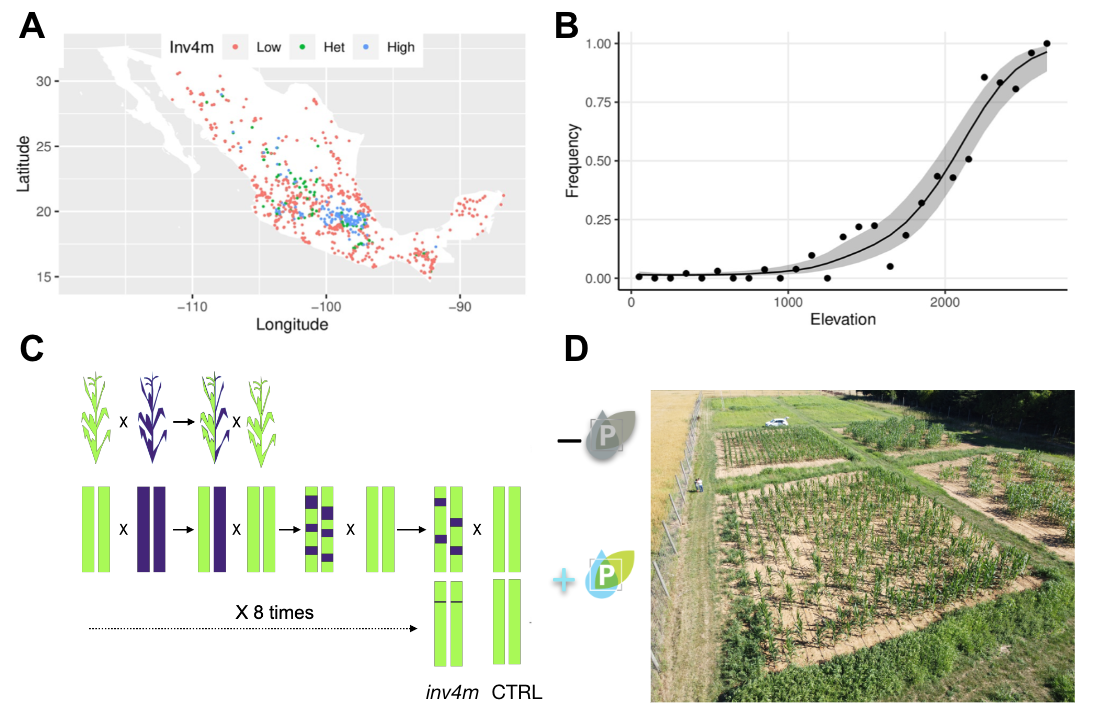
\includegraphics[width=\linewidth]{Chapter-3/figs/design.png}
\caption[\textit{inv4m} Distribution and Introgression Breeding Design]{\textit{\textbf{inv4m Distribution and Introgression Breeding Design.}}}
% \\\hspace{\textwidth} 
\textbf{(A)} 
\textbf{(B)}
\textbf{(C)} 
\textbf{(D)}
\label{fig::design}
\end{figure}

\section{Methods}
\subsection*{inv4m plant population, growth conditions,experimental design and phenotype measurements}

\subsection*{RNAseq tissue sampling, RNA extraction and Sequencing}

\subsection*{Differential Gene Expression Analysis}

%\subsection*{Gene Regulatory Network Analysis}

%\subsection*{Lipid Analysis}




% \subsection{Phosphorus response of the leaf gene regulatory network to inv4m introgrression}

\section{Results}

\subsection{Maize Vegetative and Reproductive Traits have a marked response to Phosphorus but no detectable difference between Inv4m alleles(karyotypes) nor  Inversion X Phosphorus treatment interaction}

We see a clear shoot phenotypic response to phosphorus treatment independently of Inv4m karyotype. 
Plants grown in low phosphorus grow slower and reach maturity later with a similar effect in both Inv4m and B73 homokaryotpes. 
The effect of phosphorus treatment is significant for all the vegetative growth measurements taken, plant height at anthesis, dry mass at 40, 50, 60 and 120 DAP.  
For reproductive traits low phosphorus leads to earlier time to male and female flowering, greater cob width and length, and a reduced yield as measured by total kernel weight per ear.
A closer analysis of the growth curves inferred from accumulated dry mass at different days show increased final dry mass  with increased phosphorus, a faster mass acquisition rate, and faster time to mid mass in higher phosphorus. 
There is slight evidence for an interaction between inv4m karyotype and growth. 

The standard homokaryotype (B73), seems to be more responsive to increased concentration of phosphorus in the soil. In contrast, the  inverted homokaryotype [inv4m] seems to not to lose as much dry weight in the low phosphorus treatment compared with high P input [make pairwise bootstrap test for the diference of means]. 
This behavior matches the expectation of B73 being selected for yield under high input agriculture in contrast with the Mexican Highland landraces that are selected for more predictable yields under variable stresses. In a phenotype PCA of the different mean row measurements the first dimension explaning 28\% of the variance with morphological phenotypes has weights associated with flowering time and dry mass accumulation, highlighting these variables as the most responsive to the phosphorus treatment (PCA biplot). 
The samples in this pheotypic ispace show a clear separation by treatment  but not  inv4m karyotypes ( 2 x MANOVA 2 groups) or their interaction (MANOVA 4 groups).


\begin{figure}[!ht]
\centering
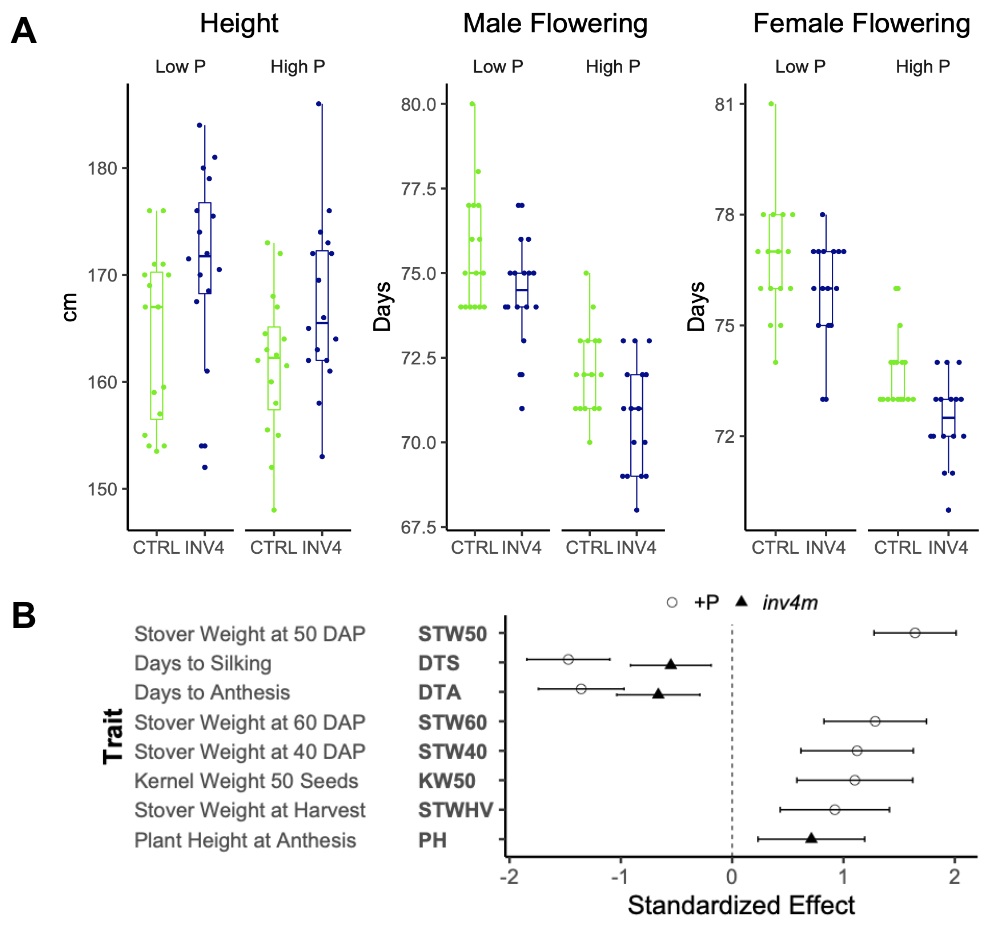
\includegraphics[width=\linewidth]{Chapter-3/figs/effects.png}
\caption[Inv4m fitness is higher independently of phosphorus treatment]{\textit{\textbf{Inv4m fitness is higher independently of Phosphorus treatment.}}}
% \\\hspace{\textwidth} 
\textbf{(A)} 
\textbf{(B)}
\label{fig::effects}
\end{figure}


\begin{figure}[!ht]
\centering
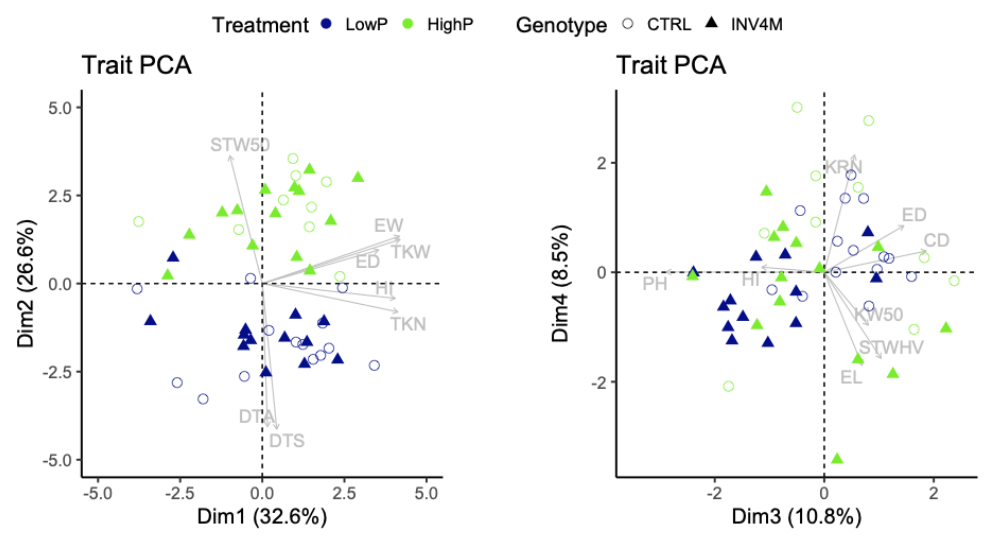
\includegraphics[width=\linewidth]{Chapter-3/figs/traitPCA.png}
\caption[The effect of Phosphorus treatment dominates phenotype differences]{\textit{\textbf{The effect of Phosphorus treatment dominates phenotype differences.}}}
% \\\hspace{\textwidth} 
\textbf{(A)} 
\textbf{(B)}

\label{fig::\textbf{(B)}}
\end{figure}

\begin{figure}[!ht]
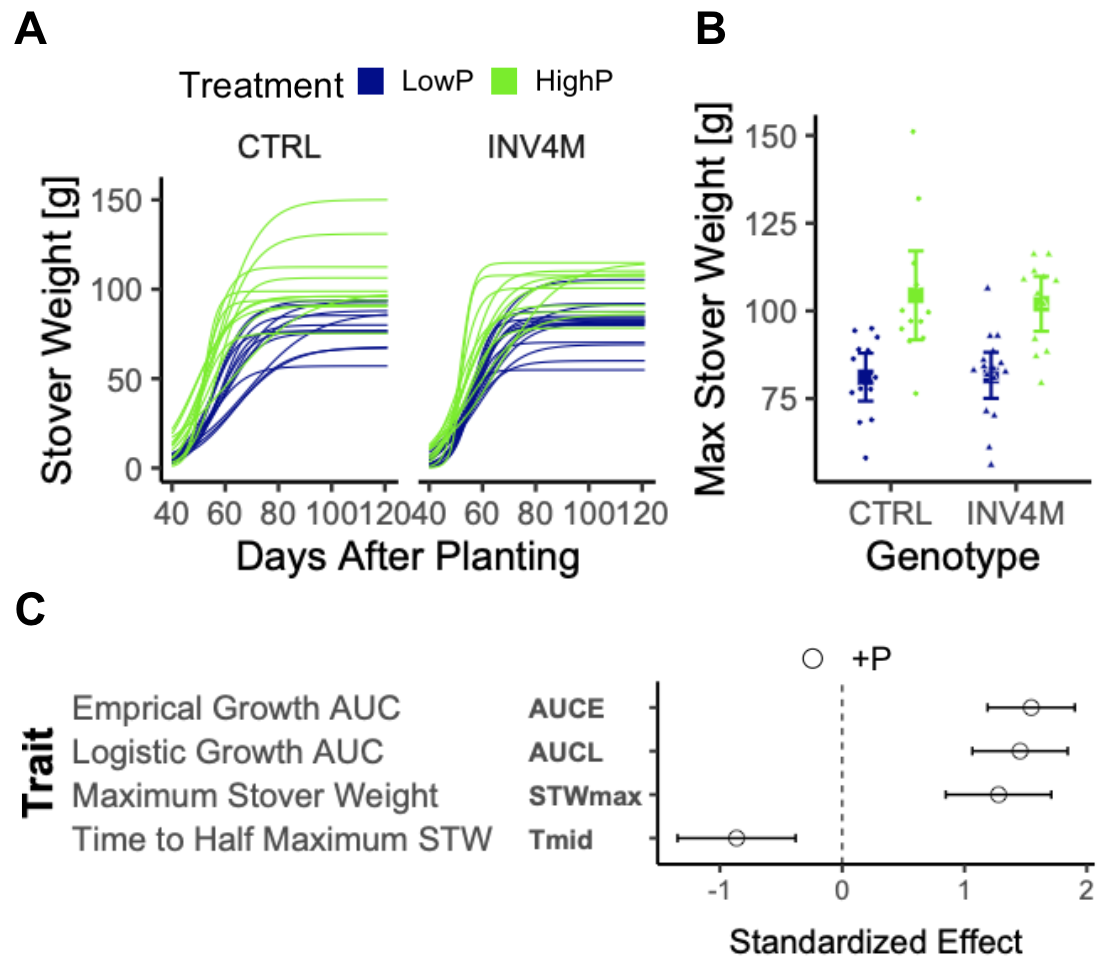
\includegraphics[width=\linewidth]{Chapter-3/figs/growth.png}
\caption[Phosphorus treatment affects growth but there is no evidence on inversion effect]{\textit{\textbf{Phosphorus treatment affects growth but there is no evidence on inversion effect.}}}
% \\\hspace{\textwidth} 
\textbf{(A)} 
\textbf{(B)}

\label{fig::\textbf{(B)}}
\end{figure}


\subsection{Maize leaf expression shows a marked response to Phosphorus and Inv4m polymorphism, with some genes responding to Inversion x Phosphorus interaction}



At v8-9 maize plants showed a remarkable response to phosphorus in their leaf gene expression.
A multidimensional scaling of the gene expression shows an overall response to phosphorus that tends to increase with leaf-age and is associated with  the first dimension (Figure). 
While the second dimension shows more separation between samples due to leaf age.

After a mashr analysis for the effects of phosphorus treatment in gene expression we see that mir399 is consistently over-expressed from the most apical to the most basal of the sampled leaves.
Gene expression on target genes like SPX transporters were also consistently diminished in high phosphorus, corresponding to the overall expected response to phosphorus (mir2020).

The phosphorus treatment has a genome-wise effect on gene expression, as shown by the mashr p-values {expression manhattan plots}. We found a total of 10000 differential expressed genes (out of 20000 genes detected in at least one leaf sample), with a distrubution mostly consistent with gene density throughout the genome. 
In contrast, the effect of inv4m is mostly detected inside the boundaries of inv4m [I need to genotype the samples  show the actual boundaries  in these plants] with a  transcription factor being the most significantly affected gene in the group (cite fold change gene id predicted function).
We detected 300 genes that undergo inv4m effect in cis, while 300 genes show significant diferential gene expression in trans between inv4m karyotypes.
The mean magnitude of the effect in cis is greater than the mean effect in trans (mean fold value of the two grops, t-tes p value (sperate hypothesis for over and under expressed genes?)).

\begin{figure}[!ht]
\centering
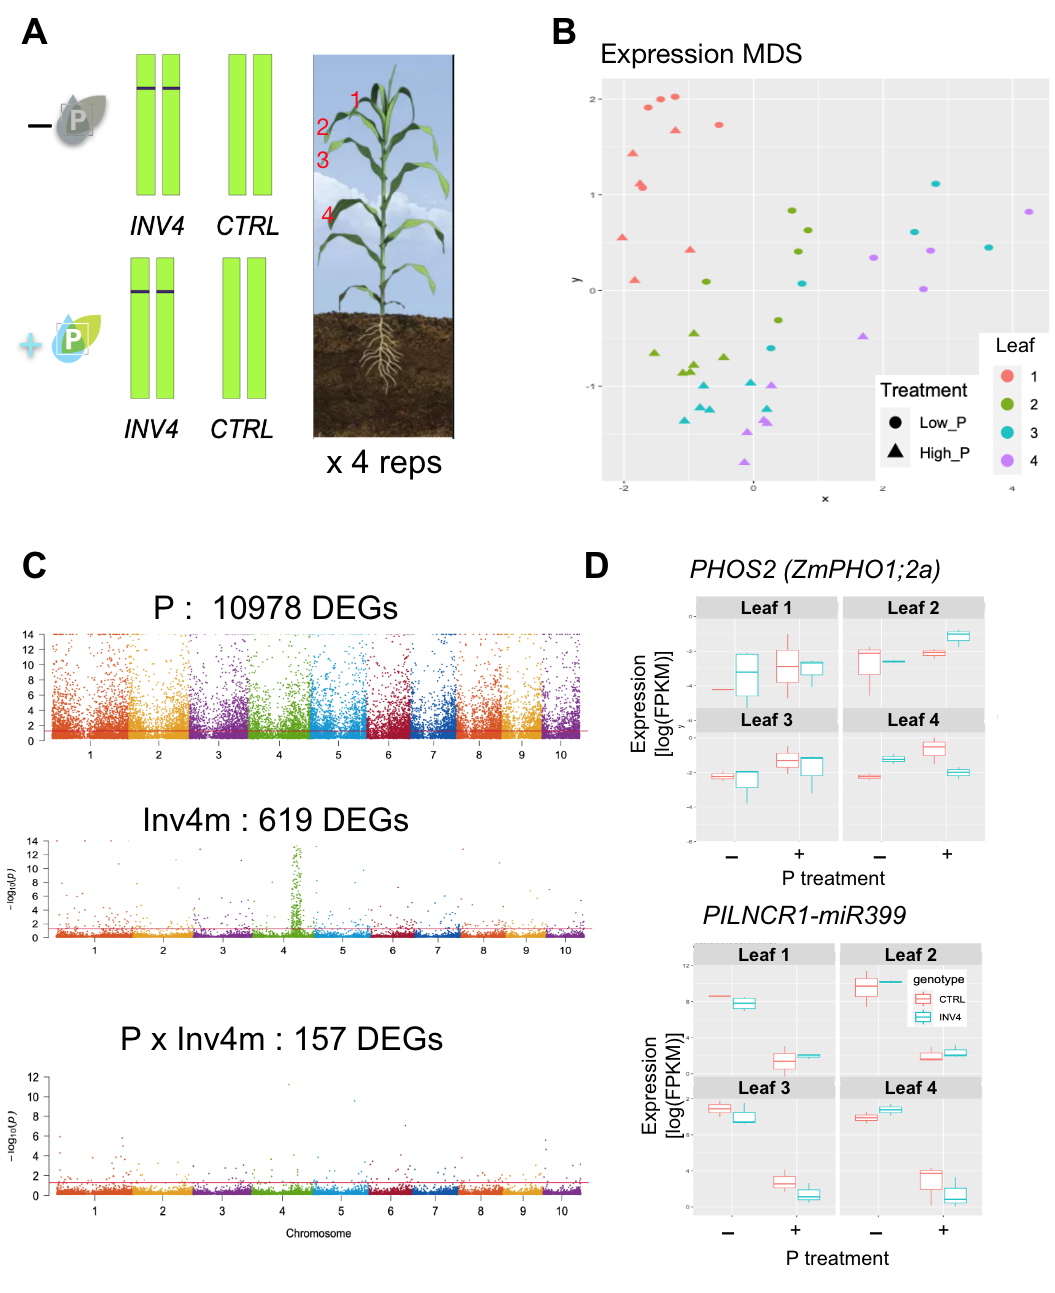
\includegraphics[width=\linewidth]{Chapter-3/figs/RNAseq.png}
\caption[Effect of Inv4m, Phosphorus Treatment and Interaction in Gene Expression]{\textit{\textbf{Effect of Inv4m, Phosphorus Treatment and Interaction in Gene Expression.}}}
% \\\hspace{\textwidth} 
\textbf{(A)} 
\textbf{(B)}
\textbf{(C)}
\textbf{(D}
\label{fig::\textbf{(B)}}
\end{figure}
\clearpage

However the variation at inv4m seems to have no major effect in the gene response to phosphorus.
As shown by the mashr test for the Inversion x Phosphorus interaction there are 150 genes that have a differential response to phosphorus depending on the inv4m karyotype, with (20) genes in cis and (x) genes in trans.
A single gene close to inv4m shows a different response  to phosphorus (look for the id, check if it is in the inv4m) depending on inv4m genotype (show interaction plot).

Gone ontology and pathway analysis. 
We observe clear over representation of nitrogen associated biological processes and metabolic pathways in  the 10000 genes responsive to phosphorus treatment.
However when we reduce he list to the top 1000 most significant, the over represented gene processes and terms are more related to phosphorus (adjusted FDR < 1e-6). 
Meaning that the genes that show the greater and/or more consistent effect  have phosphorus associated funcions while nitrogen related genes are making significant but smaller adjustments in expression (t test for difference in effects between phosphorus genes and nitrogen genes), maybe reflecting cross-talk between phosphorus and nitrogen homeostasis (i.e nutrient interaction) \citep{torres-rodriguez2021} [look for NxP imporrtant genes in vlad lists and other papers]. [I could mention the NEU results too]
[Make lists for over and under represented genes, maybe Miami plots?, a heatmap and hierarchical clustering of genes exprerssion profiles from leaf 1 to 4 might be nice use cheng li package to get a quick idea]

Genes that are deferentially expressed  due to Inv4m effect do not show over representation of either biological processes or pathways, not even when separated in induced vs repressed genes.
And, similarly, genes that show inv4m X phosphorus interaction in gene expression lack any specific functions statisttically associated either in Gene Ontology or Metabolic pathway database.

Overall there is no hard evidence from this transcriptome experiment that inv4m contributes to local adaptation to phosphorus, in the sense that it's adaptive contribution does not depend on phosphorus amount in the the soil.
However it is clear that inv4m plants reach faster time to maturity, and have less yield penalty under extreme phosphorus stress.
We could not find signals of photosynthesis or carbohydrate over representation in the Inv4m responsive to inversion karyotype, as was previously foundd in respons to cold \citep{crow2020}

\section{Discussion}
\printbibliography[heading=subbibintoc, title=References]

